%% The following is a directive for TeXShop to indicate the main file
%%!TEX root = diss.tex

\chapter{Introduction}
\label{ch:Introduction}

\begin{epigraph}
    \emph{If I have seen farther it is by standing on the shoulders of
    Giants.} ---~Sir Isaac Newton (1855)
\end{epigraph}

**First paragraph on CFD in laptop

**Second paragraph on what is mesh in laptop

The process of discretization of the domain to form the basis of solving the Navier-Stokes equations, or any other differential equation numerically is called mesh generation. Save a few exotic methods, almost all of the techniques in CFD require a mesh to solve the flow on. Traditionally, mesh generation was a very manual process, where engineers used to place the mesh points and cells by hand. Such heuristic approach to mesh generation gave them a lot of freedom in discretizing the domain. Cells could be aligned to the boundaries of objects. The quality of the cells, which was taken as some measure of the interior angle of the cells, was almost always chosen to be good. The benefits of this method were quite evident. However, there were some major drawbacks. The process of mesh generation was incredibly slow. Engineers would spend hours, sometime days to create the mesh for a given geometry. Also, mesh adaptation with solution was almost non-existant because that would have made the process even slower.

\begin{definition}
A mesh $M$ is a geometrical discretization of a domain $\Omega$ that consists of (a) a collection of mesh entities $M_i$ of controlled size and distribution and (b) topological relationships or adjacencies forming the graph of the mesh. The mesh $M$ covers $\Omega$ without neither overlap nor hole.
\end{definition}

The evolution of mesh generation can be correlated to the evolution of compute power available to the boffins. With the advent of third generation computers (1964-1971) carryinig integrated circuits, engineers were able to automate some of the manual processes in mesh generation. Meshes consisting of a template that repeats itself could be generated. These meshes were called structured meshes as their adjacencies or relationships could be known implicitly. The connectivity pattern repeats in such a mesh. Figure \ref{fig-block-structured-mesh} shows such a mesh for NACA 0012 airfoil.

\begin{figure}
  \begin{subfigure}{0.5\linewidth}
    \centering
    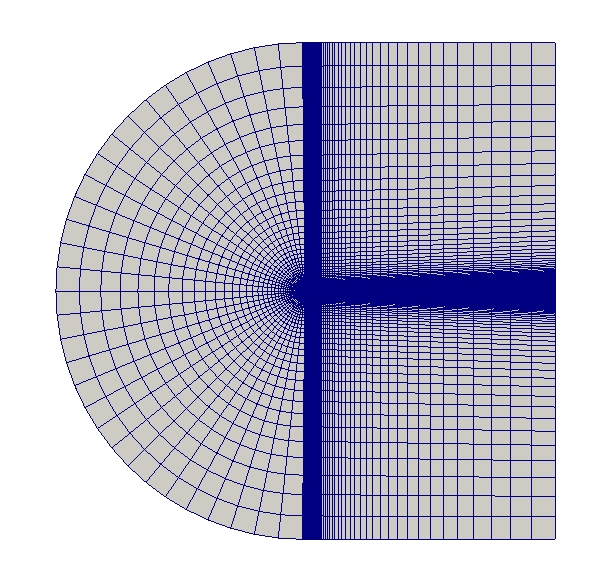
\includegraphics[width=\linewidth]{img/intro/structured.jpg}
    \caption{}
  \end{subfigure}%
  \begin{subfigure}{0.5\linewidth}
    \centering
    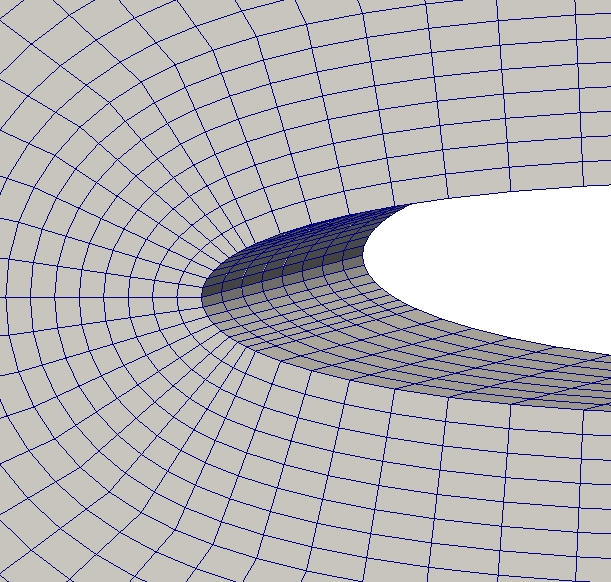
\includegraphics[width=\linewidth]{img/intro/structuredCloseUp.jpg}
    \caption{}
  \end{subfigure}%
  \caption{Block Structured Mesh of NACA 0012 airfoil. (a) Overall Mesh (b) Close Up Image of the Mesh at the leading edge of the airfoil \cite{HOPR}.}
  \label{fig-block-structured-mesh}
\end{figure}

Structured meshes were attractive to engineers because of their low memory usage because of repeated topology. Also, given simple domains to mesh, these meshes were optimal for minimizing the errors in CFD, resulting in faster simulations \cite{d1991optimal}.

\section{Boundary Layer Phenomenon}

\section{Anisotropic Meshing}

\section{Objective and Outline}